\section{Supplemental Results}
\label{a:results}
Additional information on data sources, analysis, and results are available
in the public repository:\\
\hreftt{https://github.com/mishra-lab/sr-heterogeneity-hiv-models}
% ==============================================================================
\subsection{Map}\label{aa:res:map}
\begin{figure}[H]
  \centering
  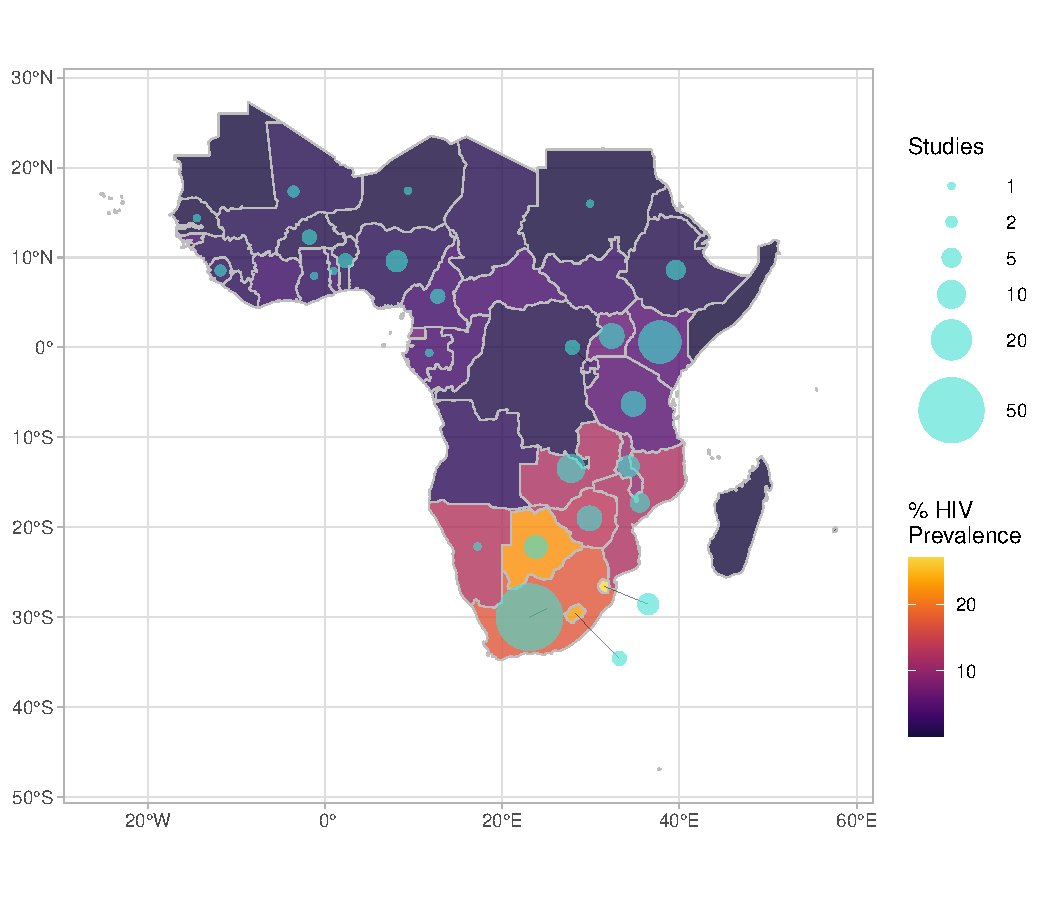
\includegraphics[width=0.8\textwidth]{map}
  \caption{Map showing number of studies (of 94 total)
    applying HIV transmission modelling in each country vs
    the number of people living with HIV (PLHIV, millions)}
  \label{fig:map}
\end{figure}
\clearpage % TEMP
% ==============================================================================
\subsection{Risk Heterogeneity}\label{aa:res:risk}
% ------------------------------------------------------------------------------
\subsubsection{Distributions}
The following figures illustrate the distributions (number of studies)
of various parameter values and modelling assumptions related to
factors of heterogeneity and intervention contexts.
\par
\foreach \var/\title in \plotlistdist{
  \begin{minipage}[t][.33\textheight][t]{0.48\linewidth}
    \includegraphics[width=0.95\textwidth]{{d.\var}.pdf}
    \captionof{figure}{\title}
    \label{fig:\var}
  \end{minipage}\hspace{0.04\linewidth}}
\clearpage
% ==============================================================================
\subsection{ART Prevention Impact}\label{aa:res:api}
The following figures illustrate the projected ART prevention impact (Dataset~B),
stratified by various factors of heterogeneity and intervention contexts (colours).
The left panels show the relative reduction in HIV incidence rate;
the right panels show the relative reduction in cumulative new HIV infections;
both as compared to a base-case scenario reflecting status quo.
The number of studies (scenarios) reporting
incidence reduction, cumulative infections averted, both, or either was:
\x{n/n.a.api.inc}~(\x{n/n.s.api.inc}),
\x{n/n.a.api.chi}~(\x{n/n.s.api.chi}),
\x{n/n.a.api.both}~(\x{n/n.s.api.both}), and
\x{n/n.a.api}~(\x{n/n.s.api}), respectively.
If any study included multiple scenarios of ART scale-up,
then each scenario was included separately,
but the size of each data point was reduced
in proportion to the number of scenarios;
so studies with only one scenario have the largest data points.
Some scenarios have multiple data points if multiple time horizons were reported.
If any factor could not be quantified due to missing data or varying values,
the data point is grey.
A small random offset has been added to the data points to reduce overlap.
\begin{figure}[H]
  \begin{subfigure}{0.5\linewidth}
    \includegraphics[width=\linewidth]{{inc.s.Risk.both}.pdf}
    \caption{Reduction in HIV incidence (\%)}
  \end{subfigure}%
  \begin{subfigure}{0.5\linewidth}
    \includegraphics[width=\linewidth]{{chi.s.Risk.both}.pdf}
    \caption{Cumulative HIV infections averted (\%)}
  \end{subfigure}
  \caption{Projected ART prevention benefits,
    stratified by factors of risk heterogeneity: whether models considered
    differences in sexual activity, key populations, and
    ART cascade prioritized to key populations.
    Subset of studies reporting both outcomes.}
  \label{fig:api:both}
\end{figure}
\foreach \var/\title in \plotlistapi{
  \begin{figure}[H]
    \begin{subfigure}{0.5\linewidth}
      \includegraphics[width=\linewidth]{{inc.s.\var}.pdf}
    \end{subfigure}%
    \begin{subfigure}{0.5\linewidth}
      \includegraphics[width=\linewidth]{{chi.s.\var}.pdf}
    \end{subfigure}
    \caption{\title}
    \label{fig:api:\var}
  \end{figure}
}
\begin{figure}[H]
  \centering
  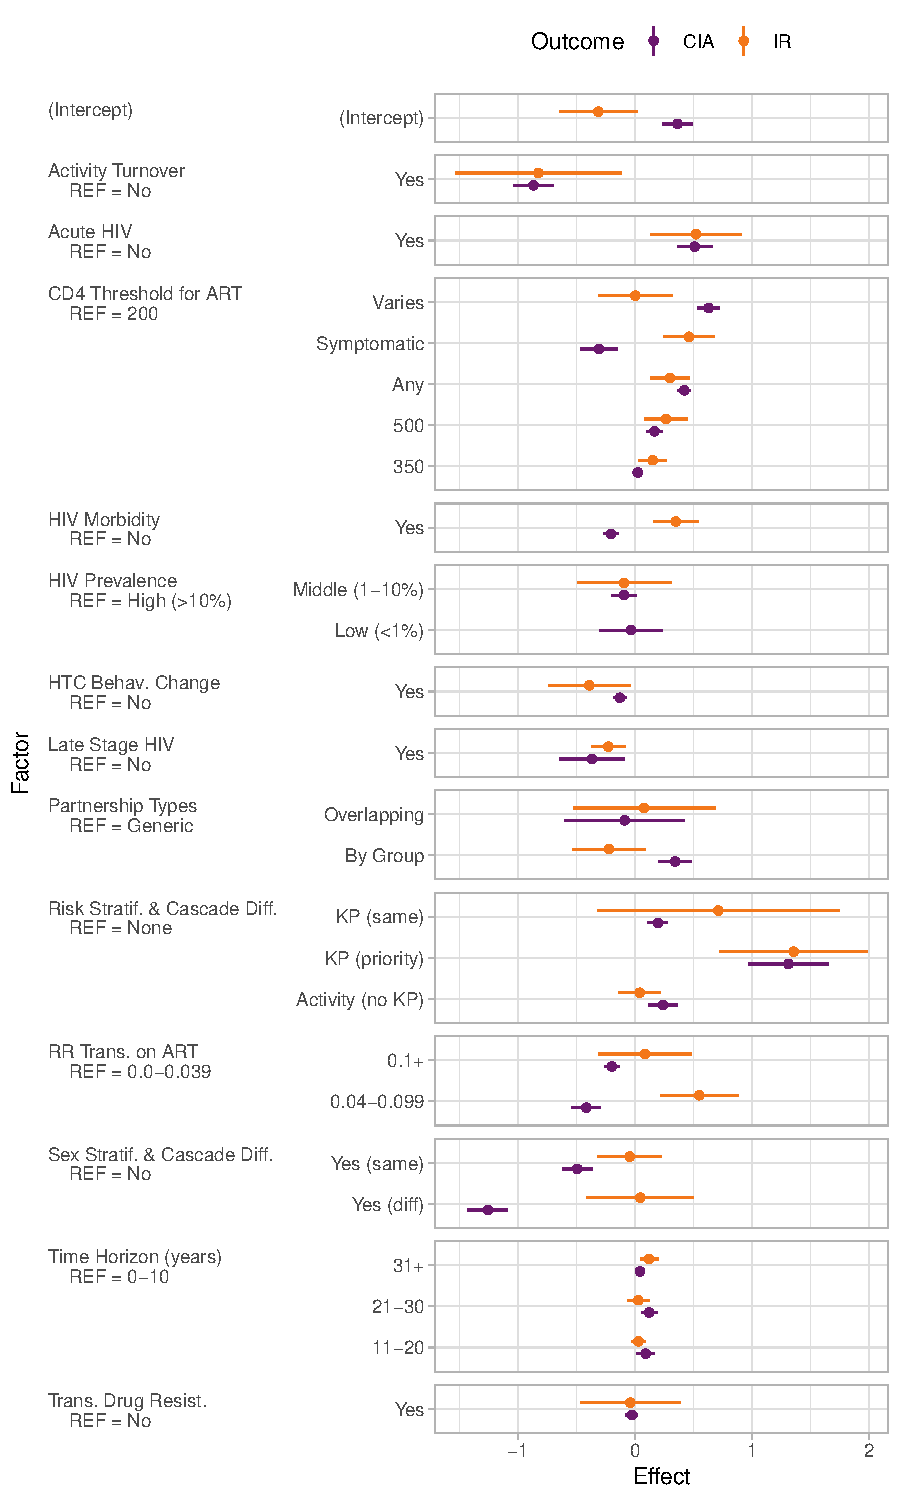
\includegraphics[width=0.75\linewidth]{effects}
  \caption{Effect estimates for factors of heterogeneity on
    incidence reduction (\%, IR) and cumulative infections averted (\%, CHI)
    from linear multivariate regression with generalized estimating equations.}
  \label{fig:effects}
  \floatfoot{
    RR: relative risk;
    HTC: HIV testing and counselling;
    KP: key populations.
    priority: modelled ART cascade transitions were faster in KP vs overall due to prioritized programs;
    same: cascade transitions were assumed the same in KP as overall.
    Factor definitions are given in Appendix~\ref{a:defs}.
  }
\end{figure}